\chapter{Quark Masses}

Quarks are not asymptotic states of nature, so their masses cannot be measured in experiments. They are generally defined in some perturbative scheme like $\overline{\mathrm{MS}}$ and at some scale $\mu$. Their values remain amongst the least well known of the Standard Model parameters. In this section I will discuss their extraction from lattice data.

The extraction of the up, down, and strange quark masses from the hadron spectrum is done by inverting Eqs.~18.3 once the coefficients $A_\pi$ etc.\ are determined from fits to the lattice data. As I have mentioned before, current lattice simulations neglect iso-spin breaking effects, so we can only determine $m = (m_u + m_d)/2$ and $m_s$. I will discuss these first and then briefly mention the extraction of the heavy quark masses $m_c$ and $m_b$.

In the quenched approximation, the most straightforward way to estimate $m$ is to extrapolate $M_\pi^2/X^2$ to the physical value. Here $X$ is a dimensionful quantity like $f_\pi$ or $M_\rho$ or $M_N$ or $M_\Delta$ that does not depend on $m_s$, and de facto sets the lattice scale $1/a$. Of the above quantities, using $M_\rho$ is the most controversial as it decays via strong interactions and has a large width, 170~MeV. On the other hand the lattice data for $M_\rho$ is most readily available and has good signal. Also, in the quenched approximation the $\rho$ does not decay. Using $M_\rho$ to set $a$ in QQCD versus some other quantity can therefore give an overall scale uncertainty. The spread in $1/a$ extracted from different quantities is found to be $\approx 10\%$, and this uncertainty, inherent to the quenched approximation, will be treated as an overall systematic error. Similarly, one can set $m_s$ by extrapolating the ratio $M_s/X$, where $M_s$ is any state that depends on $m_s$ like $M_K$, or $M_{K^*}$, or $M_\phi$ or any of the baryons containing a strange quark. The world data show that different choices of $M_s$ give rise to a $\approx 20\%$ spread in $m_s$. It is important to note that if one assumes the relation $M_{PS}^2 = B_{PS} m_q$ (which LQCD has not validated as true for the whole range $[m, m_s]$), and uses $M_K$ to fix $m_s$, then the ratio $m_s/m$ has to be 25.9 if $m$ is set using $M_\pi^2$.

In the full theory $X$ depends on $m_s$, and similarly $M_s$ depends on $m$, through sea quark effects. Thus, $m$, $a$, and $m_s$ have to be fixed by solving the coupled set of equations.

Simulations of the hadron spectrum have been done by a number of collaborations around the world, and there exists a large amount of data for the masses of hadrons as a function of the quark masses and lattice spacing. (Almost all lattice collaborations, for example the APE, Columbia University, CP-PACS, Fermilab, GF11, HEMCGC, JLQCD, Los Alamos, SCRI, staggered, UKQCD, and the Wuppertal University collaborations, have contributed to these calculations [183].) In early analyses the estimates of quark masses varied by almost a factor of two between different formulations of fermions, and the pattern of the discretization and quenching errors was not obvious from the work of any one collaboration. Clarification of this issue has been obtained by putting together all the world data for Wilson, clover, and staggered fermions [183,184]. The final picture for $m$, based on the most recent, high statistics, and large lattices data is shown in Fig.~\ref{fig:34} for the three fermion formulations. This figure shows clearly that the factor of $\sim 2$ difference at $1/a \sim 2$~GeV shrinks to $\sim 15\%$ after extrapolation to $a = 0$, i.e.\ most of the difference can be explained as due to discretization errors.

The behavior of $m_s$ versus $a$ is very similar. A summary of the quenched results in MeV at scale $\mu = 2$~GeV, based on an analysis of the 1997 world data [185], is

\begin{table}[htbp]
\centering
\begin{tabular}{lccc}
\toprule
          & $m(M_\pi)$ & $m_s(M_K)$ & $m_s(M_\phi)$ \\
\midrule
Wilson    & 4.1(1)     & 107(2)     & 139(11)       \\
TI Clover & 3.8(1)     & 99(3)      & 117(8)        \\
Staggered & 3.5(1)     & 91(2)      & 109(5)        \\
\bottomrule
\end{tabular}
\caption*{Quenched estimates of the light quark masses (in MeV), at scale $\mu = 2$~GeV, for the Wilson, tadpole improved clover (TI Clover), and staggered formulations of fermions, based on an analysis of the 1997 world data [185].}
\label{tab:light-quark-masses}
\end{table}

These estimates were obtained using the following Ans\"atze.
\begin{itemize}
\item Chiral fits were made keeping only the lowest order terms shown in Eqs.~18.3.
\item $M_\pi^2/M_\rho$ is used to fix $m$.
\item Results for $m_s$ are given for two choices, $M_K^2/M_\rho$ and $M_\phi/M_\rho$. (Using $M_{K^*}/M_\rho$ gives values almost identical to those with $M_\phi/M_\rho$. This implies that for the choice $m_s(M_\phi)$ one could equivalently have set the scale using $M_{K^*}$ instead of $M_\rho$.)
\item Since linear chiral fits have been used, $m_s(M_K) \equiv 25.9\,m$.
\item The matching factor, $Z_m$, between lattice and $\overline{\mathrm{MS}}$ schemes is the tadpole improved 1-loop result.
\item The extrapolation to $a = 0$ is done using the lowest order discretization error, i.e.\ $O(a)$ and $O(\alpha_s a)$ for Wilson and clover, and a quadratic in $a^2$ for staggered.
\end{itemize}

The final difference in estimates between Wilson, tadpole improved clover (TI Clover), and staggered results is $\approx 15\%$ as shown in Fig.~\ref{fig:34}. This could be due to the neglected higher order discretization errors and/or due to the difference between non-perturbative and 1-loop estimates of $Z$'s. Similarly, the $\approx 20\%$ variation in $m_s$ with the state used to extract it, $M_K$ versus $M_\phi$ (or equivalently $M_{K^*}$) could be due to the quenched approximation or partly an artifact of keeping only the lowest order discretization correction in the extrapolations. To disentangle these discretization and quenching errors requires precise unquenched data with roughly physical values for light quarks.

\begin{figure}[htbp]
\centering
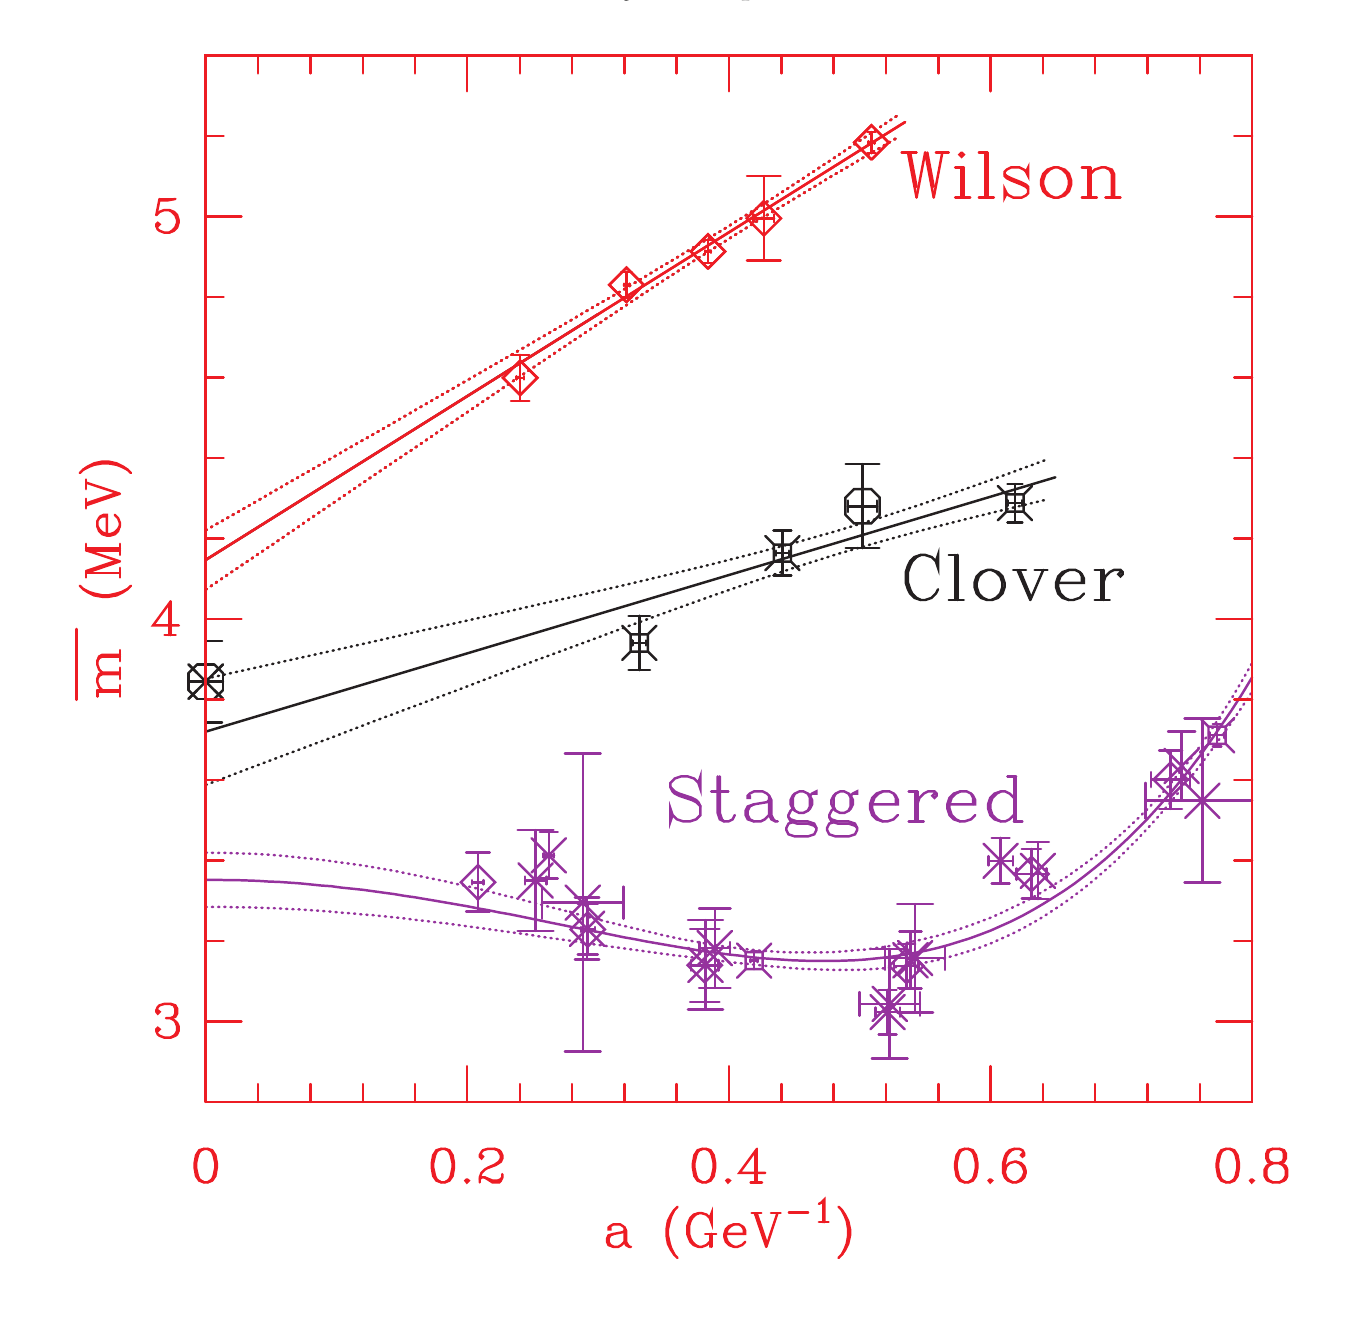
\includegraphics[width=0.8\textwidth]{images/fig34.png}
\caption{The behavior of $m_u + m_d$ as a function of the lattice spacing $a$ for three discretization schemes -- Wilson, clover, and staggered. Linear extrapolations to $a = 0$ are shown for Wilson and clover formulations, while for staggered both $O(a^2)$ and $O(a^4)$ terms are incorporated in the fit. The theoretically expected form for discretization errors in the clover formulation is $O(\alpha_s a)$. The extrapolated value using this form is shown by the symbol burst.}
\label{fig:34}
\end{figure}

For best estimates of quenched results I average the data and use the spread as the error. To these, I add a second systematic error of 10\% due to the uncertainty in the determination of the scale $1/a$, which partly reflects the uncertainty due to the quenched approximation. The results, in the $\overline{\mathrm{MS}}$ scheme and evaluated at 2~GeV, are [185]
\begin{equation}
\begin{aligned}
m &= 3.8(4)(4)~\mathrm{MeV}, \\
m_s &= 110(20)(11)~\mathrm{MeV}.
\end{aligned}
\end{equation}

\section{Light Quark Masses from Ward Identities}

A second method for extracting quark masses is based on axial and vector current Ward identities
\begin{equation}
\begin{aligned}
Z_A\,\partial_\mu A_\mu &= (m_1 + m_2)_R\, Z_P\, P, \\
Z_V\,\partial_\mu V_\mu &= (m_1 - m_2)_R\, Z_S\, S,
\end{aligned}
\end{equation}
where 1, 2 are the flavor indices and $P$ and $S$ are the lattice pseudoscalar and scalar densities. From these one can construct ratios of 2-point correlation functions
\begin{equation}
\begin{aligned}
\frac{Z_P}{Z_A}\,\frac{\langle \partial_\mu A_\mu(\tau)\,P(0)\rangle}{\langle P(\tau)P(0)\rangle} &= (m_1 + m_2)_R, \\
\frac{Z_S}{Z_V}\,\frac{\langle \partial_\mu V_\mu(\tau)\,S(0)\rangle}{\langle S(\tau)S(0)\rangle} &= (m_1 - m_2)_R,
\end{aligned}
\end{equation}
which give the renormalized quark masses once the various renormalization constants $Z_i$ are known. Since the Ward identities are operator identities, Eq.~20.3 holds for all $\tau$ except at very short times where there is influence of contact terms. Thus it is not necessary for the signal to persist to asymptotic $\tau$ as needed in spectroscopy method to isolate the lowest state.

The two estimates of quark masses, from spectroscopy and from the Ward identities, should agree in the continuum limit. A comparison of the two data sets for the Wilson action and using 1-loop perturbative $Z$'s is shown in Fig.~\ref{fig:35}. The two estimates are significantly different at finite $a$, however, a linear extrapolation works for both sets of data, and the extrapolated values are in surprisingly good agreement. One could therefore attribute the differences at finite $a$ to discretization errors.

\begin{figure}[htbp]
\centering
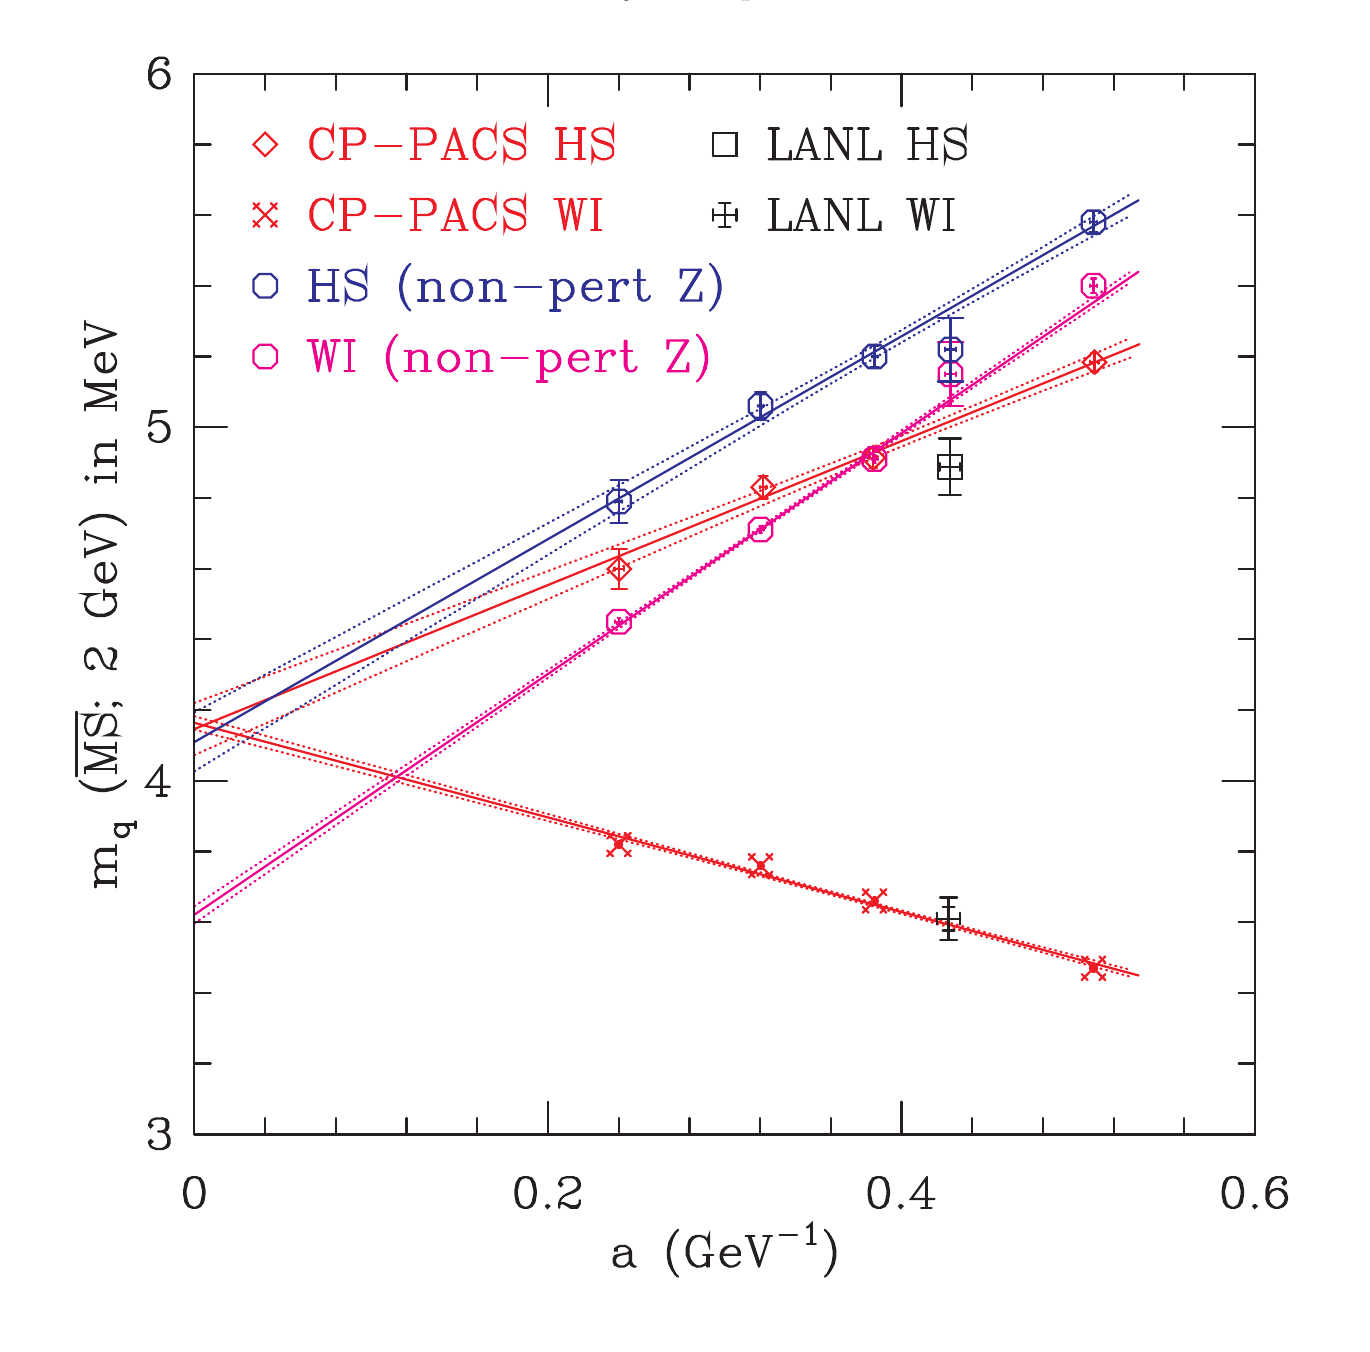
\includegraphics[width=0.8\textwidth]{images/fig35.png}
\caption{The behavior of $m = (m_u + m_d)/2$ as a function of the lattice spacing $a$ for Wilson fermions. Data from the hadron spectroscopy and Ward Identity method are shown for two ways of estimating the renormalization constants, i.e.\ one loop perturbative and non-perturbative.}
\label{fig:35}
\end{figure}

The recent non-perturbative calculations of the $Z$'s [186] challenge this nice picture. Fig.~\ref{fig:35} also shows the same data analyzed using these non-perturbative $Z$'s. At fixed $a$ the non-perturbative $Z$'s increase both the hadron spectroscopy and WI results to roughly the same value. This suggests that most of the difference is due to the $O(\alpha_s^2)$ corrections to the 1-loop $Z$'s and not due to the $O(a)$ discretization errors as mentioned before. However, the non-perturbative calculation of $Z$'s themselves have $O(a)$ errors that have not been resolved in the results of [186]. As a result we do not have a clear separation between the effects of the $O(a)$ discretization errors and the $O(\alpha_s^2)$ errors in these $Z$'s.

The bottom line is that, even though we have not resolved the two kinds of errors, and while both the value at fixed $a$ and the slope in $a$ increases significantly on changing from 1-loop to non-perturbative $Z$'s, the extrapolated value is roughly unchanged.

To conclude, I believe that we have finally obtained values for light quark masses with reliable estimates of statistical and all systematic errors other than quenching. Calculations are already underway to significantly increase the number of data points with $n_f = 2$ and 4 flavors of dynamical quarks to reduce the quenching uncertainty. Also, new ways to calculate the renormalization constants non-perturbatively are being developed. Therefore, I expect that in the next few years there will be a significant increase in the precision of both QQCD and full QCD estimates of light quark masses.

\section{Schr\"odinger Functional Approach}

In the above discussion the term non-perturbative $Z$'s referred to only the lattice scheme. In the required matching constants one still has to use perturbative expressions for the renormalization constants in the continuum scheme and make a good estimate of the matching point. The ALPHA Collaboration has proposed a method for removing this last vestige of dependence on perturbation theory [187]. The details of their method have been discussed by Prof.~L\"uscher at this school, so I will just summarize the key points.
\begin{enumerate}
\item[(i)] Calculate the quark mass using the axial WI method at some infrared lattice scale. At the same time calculate $Z_P$ and $Z_A$ non-perturbatively in the Schr\"odinger functional scheme.
\item[(ii)] Evolve this lattice result to some very high scale using the step scaling function calculated non-perturbatively.
\item[(iii)] At this high scale, where $\alpha_s$ is small, define the renormalization group independent mass
\begin{equation}
\hat{m} = \lim_{a\to 0} m_R \left[2\beta_0 g^2\right]^{-\gamma_0/2\beta_0}.
\end{equation}
\end{enumerate}
This $\hat{m}$ is scheme independent, thus subsequent conversion to a running mass in some scheme and at some desired scale can be done in the continuum using the most accurate versions (4-loop) of the scale evolution equations [188]. To reiterate, the advantage of this method is that the lattice calculations directly predict the scale and scheme invariant quantity $\hat{m}$. The calculations by the ALPHA Collaboration are still in progress and at this time estimates for $\hat{m}$ have not been released. It will be interesting to see how they compare with conventional hadron spectroscopy or WI methods discussed above. My prejudice is that they will be very similar.

\section{Role of quark masses in CP violation}

A very opportune application of the precise determination of the light quark masses is in the Standard Model prediction of direct CP violation in kaon decays characterized by the ratio $\epsilon'/\epsilon$ (see lectures by Prof.~Buras and [189]). The reason is that $\epsilon'/\epsilon$ is, to a good approximation, proportional to $1/(m_d + m_s)^2$ [190],
\begin{equation}
\epsilon'/\epsilon = A \left[c_0 + c_6 B_6^{3/2} + c_8 B_8^{3/2}\right] \left(\frac{158~\mathrm{MeV}}{m_s + m_d}\right)^2,
\end{equation}
where all quantities are to be evaluated at the scale $m_c = 1.3$~GeV. Eq.~20.5 highlights the dependence on the light quark masses and the bag parameters $B_6^{3/2}$ and $B_8^{3/2}$ which LQCD is also expected to provide. The coefficients $c_0$, $c_6$, and $c_8$ have been calculated to next-to-next-to-leading order, and with $M_{top}$ now known the main uncertainty in their extraction comes from the value of $\Lambda_{QCD}$. The quantity $A = |V_{ub}||V_{cb}| \sin\delta$ in the parameterization of Eq.~2.4, requires input of other SM parameters like $f_B$, $|V_{ub}|$, $|V_{cb}|$, $B_K$, $B_{B_d} f_{B_d}$. Using the central values quoted by Buras at scale $m_c = 1.3$~GeV [190] one gets $A = 1.29 \times 10^{-4}$, $c_0 = -1.4$, $c_6 = 7.9$, $c_8 = -4.0$. Unfortunately, the errors in these quantities make the resulting theoretical prediction, $\epsilon'/\epsilon = 3.6(3.4) \times 10^{-4}$ [190], very loose.

Current experimental estimates are $7.4(5.9) \times 10^{-4}$ from Fermilab E731 [191] and $23(7) \times 10^{-4}$ from CERN NA31 [192]. The new generation of experiments, Fermilab E832, CERN NA48, and DA$\Phi$NE KLOE, will reduce the uncertainty to $\approx 1 \times 10^{-4}$. First results from these experiments (see lectures by L.~Fayard) should be available in the next couple of years. Thus, it is very important to tighten the theoretical prediction. Clearly, lower estimates of quark masses suggested by LQCD would significantly increase the size of direct CP violation, and make its experimental determination and validation much easier.

\section{Heavy quark masses $m_c$ and $m_b$}

The masses of the heavy quarks, $m_c$ and $m_b$, have been calculated using the charmonium and upsilon spectroscopy. For heavy quarks there exist two different definitions of the quark mass --- the pole and $\overline{\mathrm{MS}}$ masses. The pole mass is defined to be $m^{(pole)} = (M_{onia} - E_{binding})/2$, where $M_{onia}$ is taken from experimental data and $E_{binding}$ is calculated on the lattice. This calculation has been done using two approaches, NRQCD [193] and heavy quark effective theory (HQET) [194], and the results are consistent. The $\overline{\mathrm{MS}}$ mass, which has the advantage of being free of renormalon ambiguities that are inherent in $m^{(pole)}$, is obtained from $m^{(pole)}$ using perturbation theory. The present results are
\begin{equation}
\begin{aligned}
m_b^{\overline{\mathrm{MS}}} &= 4.15(5)(20)~\mathrm{GeV} && \text{(APE)}, \\
m_b^{\overline{\mathrm{MS}}} &= 4.16(15)~\mathrm{GeV} && \text{(NRQCD)}.
\end{aligned}
\end{equation}
These estimates are consistent with determinations from other non-lattice methods.

The agreement is not as good for various lattice estimates of $m_c^{\overline{\mathrm{MS}}}$. Current estimates lie between $1.2 - 1.5$~GeV. For example, three different methods investigated by the APE collaboration [195,186], Fermilab collaboration [196,197], and by Bochkarev and Forcrand [198] who evaluate the correlation functions arising in QCD sum-rules on the lattice, give
\begin{equation}
\begin{aligned}
m_c^{\overline{\mathrm{MS}}} &= 1.525(40)(125)~\mathrm{GeV} && \text{(APE)}, \\
m_c^{\overline{\mathrm{MS}}} &= 1.33(8)~\mathrm{GeV} && \text{(Fermilab)}, \\
m_c^{\overline{\mathrm{MS}}} &= 1.22(5)~\mathrm{GeV} && \text{(B\&F)}.
\end{aligned}
\end{equation}
At this stage I do not consider the difference significant as the various systematic errors have not been resolved equally well in all the calculations.

\section*{Conclusions and Acknowledgements}

I hope that these lectures succeed in providing a pedagogical introduction to Lattice QCD, and to the analyses of numerical data. Undoubtedly, some topics have been left out and many are sketchy. My purpose was to give a broad overview. I have concentrated on providing the basics and have illustrated the analyses of Monte Carlo data by the calculations of the hadron spectrum, strong coupling constant $\alpha_s$, and quark masses. Prof.~Martinelli will, among other things, discuss the extraction of matrix elements of weak Hamiltonian, while Prof.~L\"uscher will provide a panoramic view of what future calculations will look like and the improvement possible with better discretization schemes. Together, I hope these set of lectures provide sufficient details and excitement to motivate some of you to probe deeper into the field.

I express my gratitude to all the lecturers, students, and staff who made this Les Houches school fun and exciting. It, most certainly, was a memorable six weeks for me. In preparing these lectures I would like to thank G.~Bali, U.~Heller, C.~Michael, M.~Peardon, the CP-PACS collaboration, in particular S.~Hashimoto and T.~Yoshie, for providing unpublished data. Special thanks go to my collaborators T.~Bhattacharya, D.~Daniel, G.~Kilcup, A.~Patel, and S.~Sharpe from whom I have, over the years, learned so much. Finally, I would like to thank T.~Bhattacharya, D.~Daniel, W.~Lee, and S.~Sharpe for proof reading these notes and for their suggestions.
